\clearpage
\section{setup}
\label{sec:setup}

\begin{SCfigure}
    \centering
    \caption{Schematic figure of the experimental setup. The
    signal processing is as following: The ionization detector
    (for a detailed description, see subsection~\ref{subsec:detector} 
    in the theoretical part) detects a potential difference within its
    condensator, passing the signal to the preamplifier (the preamplifier
    functions at the same time as a gateway of the high voltage providing
    the ionization detector). The preamplifier passes the signal to the
    main amplifier. At this point, the signal will be split and passed along
    both to the single channel analyzer (SCA) and the oscilloscope. This setup
    allows to calibrate the amplifier and the SCA depending on different
    signal strengths.
    }
    \includegraphics[width=0.5\linewidth]{figures/setup}
    \label{fig:setup1}
\end{SCfigure}

For schematic figure of the experimental setup along with a comprehensive
description see \textbf{figure~\ref{fig:setup1}}. In order to measure the activity of
the radiactive preperation we insert it inside of the ionization detector (see figure~\ref{fig:detector}) with
help of a turntable consisting of several chambers. The signal processing is now
accomplished using several devices: 
\begin{enumerate}
\item The methane of the ionization chamber 
interacts with the radiation emitted, which yields a potential difference
at the condensator (for a detailed description, 
see subsection~\ref{subsec:detector}
in the theoretical part).
\item The \textit{preamplifier} converts the current pulses into voltage pulses
and smoothes appropriately
\item After the signal is passed along to the main amplifier. The signal
will be integrated within a time span (\textit{shaping time}) which we can
choose before. The output are rectangular shaped pulses with a specific 
height, depending on the integration. These pulses are visualized at the
oscilloscope while part of the signal is passed along to the following devices.
\item The \textit{SCA} is a logical gate, selecting only those pulses which
are above a certain chosen limit. These will will be counted; this number is
our main measured quanitity and can be visualized through the computer.
\end{enumerate}
\begin{figure}[H]
    \centering
    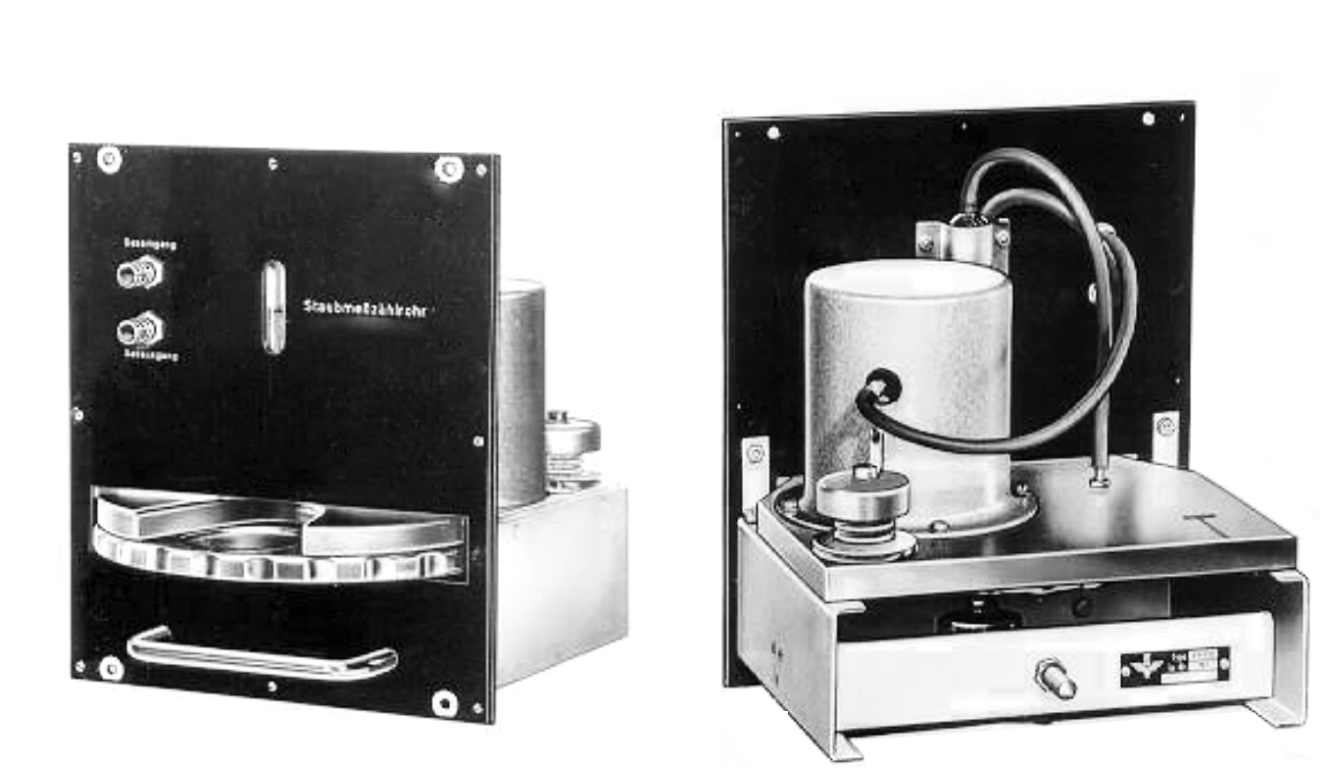
\includegraphics[width=0.6\linewidth]{figures/detector}
    \caption{Schematic figure of the methane-flow detector we are using in our experiment (from\cite{ver}).
    }
    \label{fig:detector}
\end{figure}

\subsection{procedure}
We use a ionization detector which is dependent on the continuos supply of 
gas using a gas conduit, which has to be halted when exchanging the radiative
preperation. The continuos supply of gas can be controlled by the number of
bubbles, which could be seen from a glas window. 
We used a supply with 5 bubbles / second, which was recommended in \cite{ver}.\\
The procedure is as follows:  
\begin{enumerate}
\item In order to examine the ionization detector with a highly radiactive 
preperation for calibration, we use natural uran $\mathrm{~^{238}_{92}U}$.
Since uran is both radiactive in $\alpha$ and $\beta$ rays, this can be used
to estimate both of the plateaus (which were explained in the theoretical section,
refer to subsection~\ref{subsec:plateaus}).
\item For a good estimation of the experimental background we conducted a measurement
without any radiactive preperation; only the radiation from outside and local fluctuations
will contribute to the signal.
\item Measuring samarium, we first vary the voltage in a specific range in order to 
see the $\alpha$ plateau for samarium. This is used for finding a good working point in the middle
of the plateau. This particular working point wil be used for a longer measurement, which will lead to our main result,
the activity. \label{item:samarium}
\item Point~\ref{item:samarium} will be repeated for potassium, but instead of the $\alpha$ plateau
we the potassium will yield the $\beta$ plateau, the respective steps are analogously. 
\item Again we need a good estimate for the background, therefore we will conduct a background measurement
without sample, one for each of the two working points.
\end{enumerate}
In the following we will give detailed description of out actual measurements, following the 
stated procedure. 
